% 文档类
\documentclass[12pt,a4paper]{article}

% ==== 导言区 ====
% 1. 宏包区
\usepackage{ctex} % 中文支持宏包
\usepackage{amsmath} % 数学符号支持
\usepackage{braket} % 狄拉克符号支持
\usepackage[]{graphicx} % 基本图形支持
\usepackage{float} % 浮点体的位置控制
\usepackage[most]{tcolorbox} % 笔记框制作所需宏包

% 2. 页面设置

% 3. 自定义命令区
\newcommand{\dd}{\mathrm{d}}
\newcommand{\ii}{\mathrm{i}}
\newcommand{\ee}{\mathrm{e}}

% 定义一个简单的笔记框样式
\newtcolorbox{blackbox}{
    colback=black!5!white,    % 背景色：5%黑，即很浅的灰色
    colframe=black,           % 框线颜色：黑色
    boxrule=1pt,              % 框线粗细    
    arc=4pt,                  % 圆角半径
    left=6pt, right=6pt, top=6pt, bottom=6pt, % 内边距
    boxsep=5pt,               % 内容与边框的距离
    breakable,                % 允许跨页分割（简写形式）
    enhanced,                 % 启用增强模式以获得更好的分页控制
    % 以下为新增的分页控制参数
    before skip=12pt,         % 框前间距（垂直）
    after skip=12pt,          % 框后间距（垂直）
    parbox=false,             % 不使用parbox，解决高度计算问题
    enlarge top initially by=0pt,    % 初始顶部扩展
    enlarge bottom finally by=0pt,   % 最终底部扩展
    enlarge left by=0pt,      % 左侧扩展
    enlarge right by=0pt,     % 右侧扩展
    % 调整分页处的外观
    overlay first={
        \draw[black, line width=1pt] 
            ([xshift=4pt]frame.north west) -- ([xshift=-4pt]frame.north east);
    },
    overlay last={
        \draw[black, line width=1pt] 
            ([xshift=4pt]frame.south west) -- ([xshift=-4pt]frame.south east);
    }
}

% 4. 信息填充
\title{\LaTeX 规范代码实例}
\author{SLNALS}
\date{\today}

% ==== 正文区 ====
\begin{document}

\maketitle % 信息填充部分打印

\tableofcontents % 目录打印

\section{实例内容}

本文是一个\LaTeX 文件在Vscode中配置环境后的测试效果。同时，本文也是一个代码规范的示例，后续代码的编写请严格遵照本代码的写作规范，以确保代码的可读性。
下面将展示一些例子。
\begin{equation}
    \mathbf{F} = m \frac{\dd\mathbf{v}}{\dd t}
\end{equation}
这段代码中对“，”字符存在警告，编译器认为我们在编写代码时可能混淆了全角字符和半角字符，我们可以主动忽略这一黄色框选标记。

在宏包区我们引入了支持狄拉克符号的宏包，这里有一个量子力学公式用来展示这个宏包的效果：
\begin{equation}
    \ket{\psi} = \sum_{n=1}^{N} c_n \Ket{n}
\end{equation}
需要说明的是，我们原先的配置文件并不能自动完成第三方宏包的悬停渲染，但通过在setting.json文件中添加代码可以实现这一点。可以将鼠标悬停在“equation”上面来预览加入新宏包下的公式渲染。

接着我们再看一个列表的例子：
\begin{equation}
    A = \left(
    \begin{array}{c|c}
        a_{11} & a_{12} \\ \hline % 在该行和下一行之间添加一条从左到右的横线
        a_{21} & a_{22}
    \end{array}
    \right)
\end{equation}

图片的嵌入通常可以使用下面的方法：
\begin{figure}[htbp!] % "!"必须保留，它代表忽略一些限制从而更容易排在bottom处。h=here, t=top, b=bottom, p=newpage.
    \centering
    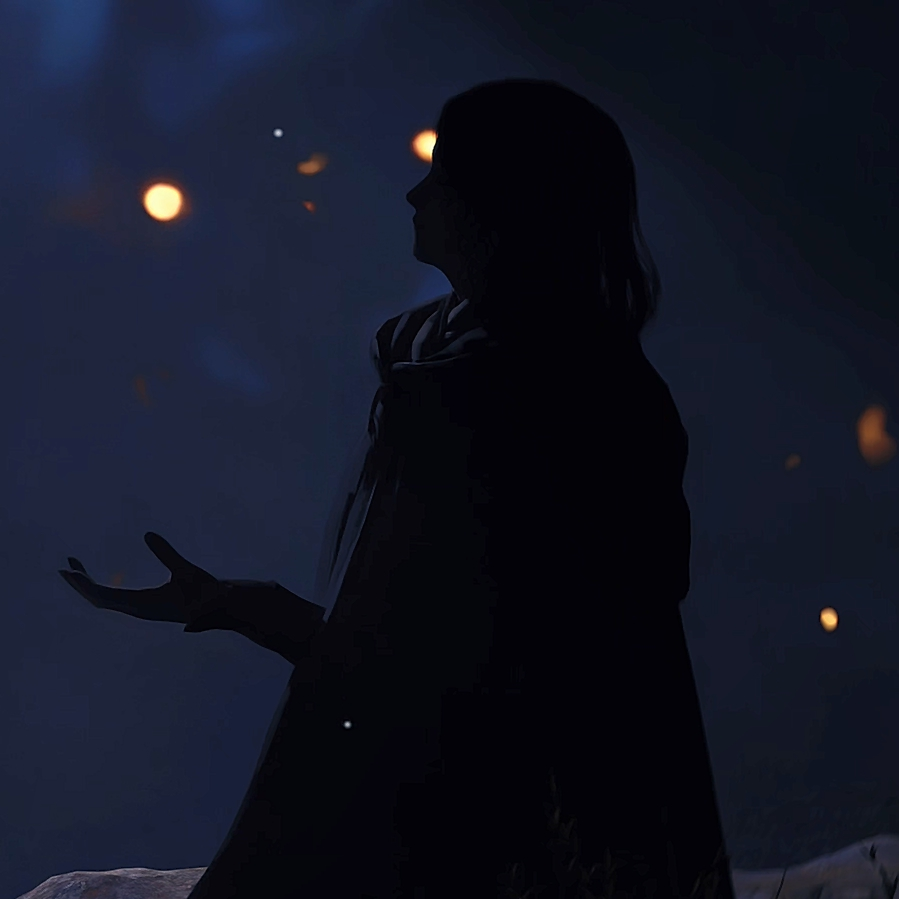
\includegraphics[width=0.4\textwidth]{figure/preview.jpg}
    \caption{Melina}
    \label{Melina}
\end{figure}

最后我们制作一个笔记框作为后续的基础工具。详细代码在导言区可查看，这里展示其效果。
\begin{blackbox}
    我们使用这样特点鲜明的文本框插入到文中以作为正文的笔记，补充等内容。
\end{blackbox}
到此我们完成了基础模板的书写，当然这只是一个不完整的例子，其余部分留待后续补充。

在此祝愿本项目能顺利完成。

\end{document}